\documentclass[12pt,compress,ngerman,utf8,t]{beamer}
\usepackage[ngerman]{babel}
\usepackage{calc}
\usepackage{ragged2e,wasysym,multicol,mathtools}
\usepackage[protrusion=true,expansion=true]{microtype}
\usepackage{tikz}
\hypersetup{colorlinks=true}

\graphicspath{{images/}}

\title{\large Wie vollbringen künstliche Intelligenzen das Kunststück des Lernens?}
\author[Ingo Blechschmidt]{\textcolor{white}{Ingo Blechschmidt \\ \small mit Dank an
Tim Baumann und Philipp Wacker}}
\date[2017-04-22]{\vspace*{-5em}\ \\\textcolor{white}{\scriptsize Institut für
Mathematik der Universität Augsburg \\ 16. Augsburger Linux-Infotag am 22. April 2017 \\}}

\useinnertheme[shadow=true]{rounded}
\useoutertheme{split}
\usecolortheme{orchid}
\usecolortheme{whale}
\setbeamerfont{block title}{size={}}

\useinnertheme{rectangles}

\usecolortheme{seahorse}
\definecolor{mypurple}{RGB}{150,0,255}
\setbeamercolor{structure}{fg=mypurple}
\definecolor{myred}{RGB}{150,0,0}
\setbeamercolor*{title}{bg=myred,fg=white}
\setbeamercolor*{titlelike}{bg=myred,fg=white}

\usefonttheme{serif}
\usepackage[T1]{fontenc}
\usepackage{libertine}

\renewcommand{\_}{\mathpunct{.}\,}
\newcommand{\BB}{\mathbb{B}}
\newcommand{\M}{\mathcal{M}}
\newcommand{\R}{\mathrm{R}}
\newcommand{\NN}{\mathbb{N}}
\newcommand{\RR}{\mathbb{R}}

\setbeamertemplate{navigation symbols}{}

\setbeamertemplate{title page}[default][colsep=-1bp,rounded=false,shadow=false]
\setbeamertemplate{frametitle}[default][colsep=-2bp,rounded=false,shadow=false,center]

\newcommand{\hil}[1]{{\usebeamercolor[fg]{item}{\textbf{#1}}}}
\setbeamertemplate{frametitle}{%
  \vskip1em%
  \leavevmode%
  \begin{beamercolorbox}[dp=1ex,center]{}%
      \usebeamercolor[fg]{item}{\textbf{\textsf{\Large \insertframetitle}}}
  \end{beamercolorbox}%
}

\setbeamertemplate{footline}{%
  \leavevmode%
  \hfill%
  \begin{beamercolorbox}[ht=2.25ex,dp=1ex,right]{}%
    \usebeamerfont{date in head/foot}
    \insertframenumber\,/\,\inserttotalframenumber\hspace*{1ex}
  \end{beamercolorbox}%
  \vskip0pt%
}

\newcommand{\backupstart}{
  \newcounter{framenumberpreappendix}
  \setcounter{framenumberpreappendix}{\value{framenumber}}
}
\newcommand{\backupend}{
  \addtocounter{framenumberpreappendix}{-\value{framenumber}}
  \addtocounter{framenumber}{\value{framenumberpreappendix}}
}

\setbeameroption{show notes}
\setbeamertemplate{note page}[plain]

\newcommand{\imgslide}[3]{{\usebackgroundtemplate{\parbox[c][\paperheight][c]{\paperwidth}{\centering\includegraphics[width=\paperwidth]{#1}}}\begin{frame}[plain,b]\tiny Quelle: \href{#2}{#3}\par\end{frame}}}

\newcommand{\portrait}[4]{\begin{column}{#3\textwidth}\centering\includegraphics[height=#4\textheight]{#1}\\{\scriptsize #2\par}\end{column}}

\begin{document}

% https://static2.gamespot.com/uploads/original/1557/15576725/2944861-hogwarts.jpg
{\usebackgroundtemplate{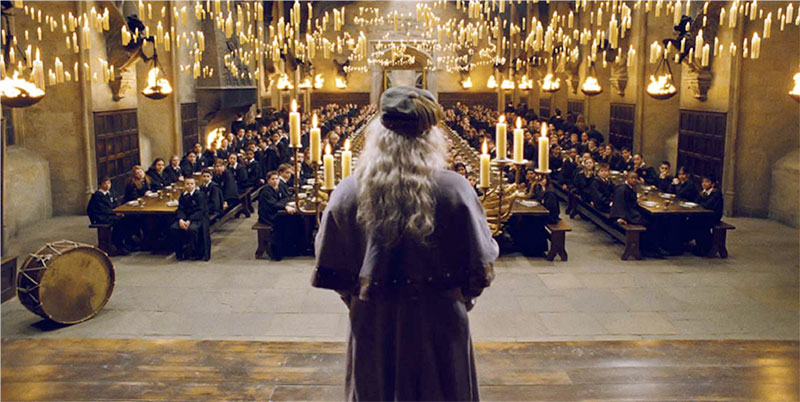
\includegraphics[height=\paperheight]{hogwarts}}
\frame{\vspace*{9em}\titlepage}}
\frame{\tableofcontents}

% Einführungsvideos
% * https://www.youtube.com/watch?v=MzJ0CytAsec
%   Windows Vista Speech Recognition Tested - Perl Scripting
% * https://www.youtube.com/watch?v=M1ONXea0mXg
%   Hound Internal Demo

\section{Erfolge von KI}

\begin{frame}
  \centering
  \bigskip\bigskip

  \Huge \hil{Teil I}

  \bigskip
  \Large\textbf{Jüngste Erfolge von \\ künstlicher Intelligenz}
  \par

  \vfill
  \vfill
  \vfill
  \begin{columns}
    % http://nerdist.com/wp-content/uploads/2016/03/DeepMind-Sedol-Go-Match-Feature-Image-03082016.jpg
    \portrait{wavenet}{\href{https://deepmind.com/blog/wavenet-generative-model-raw-audio/}{Sprachsynthese}}{0.17}{0.25}
    \portrait{deepmind-match}{\href{https://de.wikipedia.org/wiki/AlphaGo}{AlphaGo}}{0.25}{0.25}
    \portrait{neural-style}{\href{https://github.com/jcjohnson/neural-style}{Stiltransfer}}{0.25}{0.25}
    \portrait{magenta-jam-session}{\href{https://magenta.tensorflow.org/blog/2016/12/16/nips-demo/}{Jammen mit Magenta}}{0.25}{0.25}
  \end{columns}
\end{frame}

% Für Wavenet abspielen: resources/speaker-*.wav
% Für Stiltransfer: resources/jcjohnson*.html
% Für die Supervergrößerung: resources/neural-enhance.gif


\section[Wie?]{Funktionsweise künstlicher neuronaler Netzwerke}

{\usebackgroundtemplate{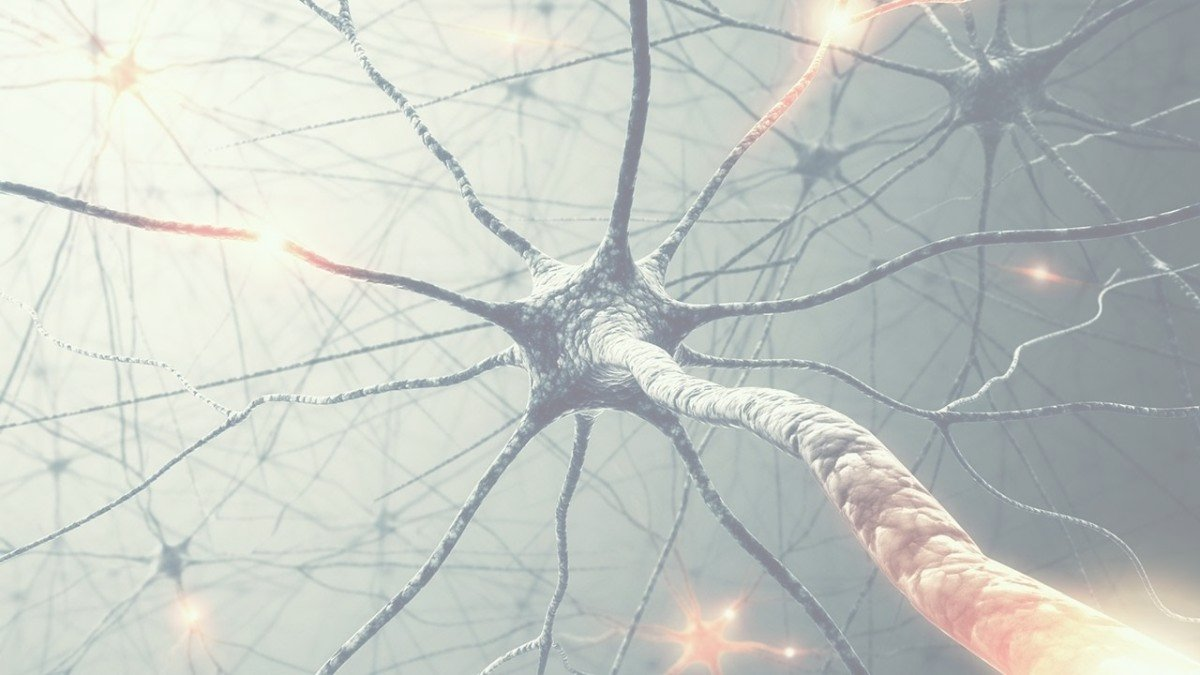
\includegraphics[height=\paperheight]{neuron-art}}
\begin{frame}
  \centering
  \bigskip\bigskip

  \Huge \hil{Teil II}

  \bigskip
  \Large\textbf{Funktionsweise künstlicher neuronaler Netzwerke}
  \par

  \vfill\small
  \begin{enumerate}
    \item Aufbau eines einfachen Netzes
    \item Bewertung durch eine Kostenfunktion
    \item Fehlerminimierung mittels Gradientenabstieg
  \end{enumerate}
\end{frame}}


\begin{frame}{Der MNIST-Datensatz}
  \centering
  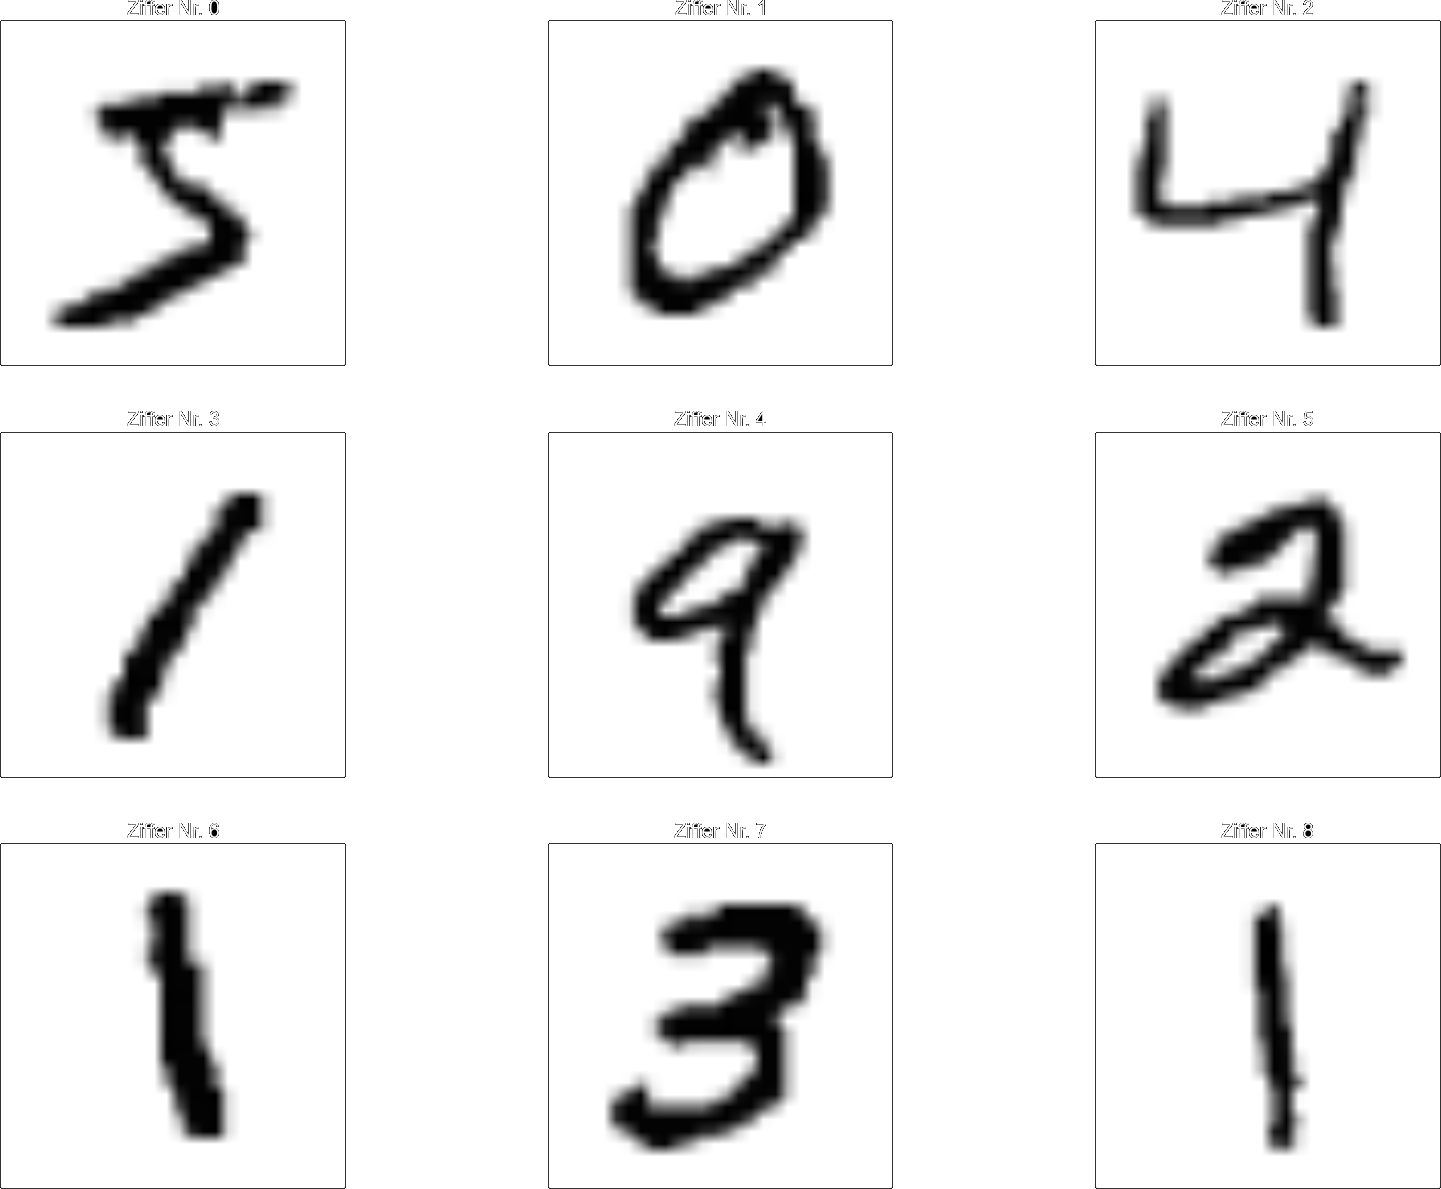
\includegraphics[width=0.7\textwidth]{mnist-ziffern}
  \bigskip

  70\,000 Bilder mit je $28 \times 28$ Pixeln
  \par
\end{frame}


\subsection{Netzaufbau}

% Vorlage von Kjell Magne Fauske, http://www.texample.net/tikz/examples/neural-network/
\begin{frame}{Aufbau eines einfachen Netzes}
  \def\layersep{2cm}
  \begin{tikzpicture}[shorten >=1pt,->,draw=black!50, node distance=\layersep]
    \tikzstyle{every pin edge}=[<-,shorten <=1pt]
    \tikzstyle{every node}=[font={\small}]
    \tikzstyle{neuron}=[circle,fill=black!25,minimum size=17pt,inner sep=0pt]
    \tikzstyle{input neuron}=[neuron, fill=green!80];
    \tikzstyle{output neuron}=[neuron, fill=red!50];
    \tikzstyle{hidden neuron}=[neuron, fill=blue!50];
    \tikzstyle{annot} = [text width=4em, text centered]

    \node[input neuron, pin=left:Eingabe 1] (I-1) at (0,-1.2*1) {\only<3->{$0{,}1$}};
    \node[input neuron, pin=left:Eingabe 2] (I-2) at (0,-1.2*2) {\only<3->{$0{,}7$}};
    \node[input neuron, pin=left:Eingabe 3] (I-3) at (0,-1.2*3) {\only<3->{$0{,}2$}};
    \node[input neuron, pin=left:Eingabe 4] (I-4) at (0,-1.2*4) {\only<3->{$0{,}4$}};

    \foreach \name / \y in {1,...,5}
      \path[yshift=0.5cm]
        node[hidden neuron] (H-1-\name) at (\layersep,-1.2*\y cm) {};
    \foreach \name / \y in {1,...,5}
      \path[yshift=0.5cm]
        node[hidden neuron] (H-2-\name) at (2*\layersep,-1.2*\y cm) {};

    \only<5->{
      \node at (H-1-2) {$y$};
    }

    \node[output neuron,pin={[pin edge={->}]right:Ausgabe 1}, right of=H-2-2] (O-1) {};
    \node[output neuron,pin={[pin edge={->}]right:Ausgabe 2}, right of=H-2-4] (O-2) {};

    \only<1>{
      \foreach \source in {1,...,4}
        \foreach \dest in {1,...,5}
          \path (I-\source) edge (H-1-\dest);
    }
    \only<2->{
      \foreach \source in {1,...,4}
        \foreach \dest in {2}
          \path (I-\source) edge (H-1-\dest);
    }
    \only<4->{
      \path (I-1) -- (H-1-2) node[midway] {3};
      \path (I-2) -- (H-1-2) node[midway] {4};
      \path (I-3) -- (H-1-2) node[midway] {1};
      \path (I-4) -- (H-1-2) node[midway] {5};
    }
    \only<1>{
      \foreach \source in {1,...,5}
        \foreach \dest in {1,...,5}
          \path (H-1-\source) edge (H-2-\dest);
    }
    \only<2->{
      \foreach \source in {2}
        \foreach \dest in {1,...,5}
          \path (H-1-\source) edge (H-2-\dest);
    }

    \foreach \source in {1,...,5}
      \path (H-2-\source) edge (O-1);
    \foreach \source in {1,...,5}
      \path (H-2-\source) edge (O-2);

    \node[annot,above of=H-1-1, node distance=1cm] (hl1) {Verborgene Schicht};
    \node[annot,above of=H-2-1, node distance=1cm] (hl2) {Verborgene Schicht};
    \node[annot,left of=hl1] {Eingabe\-schicht};
    \node[annot,right of=hl2] {Ausgabe\-schicht};

    \only<5->{
      \node[below of=O-2] (y) {\scriptsize $y = \sigma(0{,}1\cdot3 + 0{,}7\cdot4 + 0{,}2\cdot1 + 0{,}4\cdot5 + b)$};
      \draw[<-, in=120] (H-1-2.east)++(-0.1cm,0cm) to (y.west);
    }

    \only<5->{
      \node at (7.5,-1.2*4.5) {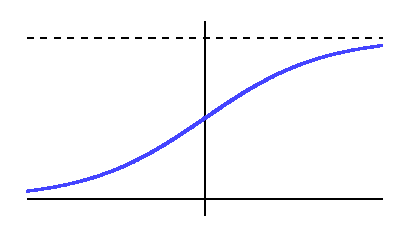
\includegraphics[scale=0.4]{sigmoid}};
    }
  \end{tikzpicture}
\end{frame}


\subsection{Lernen durch Gradientenabstieg}

\begin{frame}{Das Kunststück des Lernens}
  \centering
  \only<1>{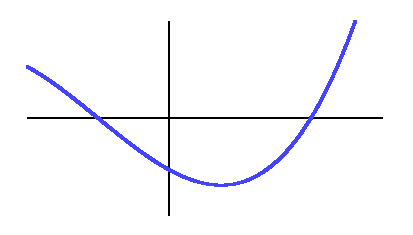
\includegraphics[width=0.8\textwidth]{cubic-polynomial} \par eine Unbekannte: $x$}
  \only<2>{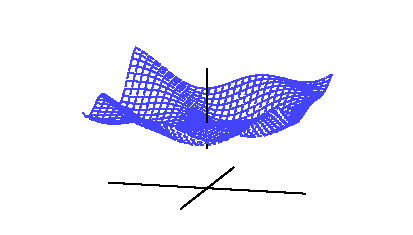
\includegraphics[width=1.0\textwidth]{3d-plot} \par zwei Unbekannte: $x$, $y$}
  \only<3>{
    \begin{columns}
      \portrait{leibniz}{\href{https://de.wikipedia.org/wiki/Gottfried_Wilhelm_Leibniz}{Leibniz (* 1646, † 1716)}}{0.3}{0.5}
      \portrait{newton}{\href{https://de.wikipedia.org/wiki/Isaac_Newton}{Newton (* 1643, † 1727)}}{0.3}{0.5}
    \end{columns}
    \bigskip

    beliebig viele Unbekannte
    \bigskip
  }
  \par
\end{frame}

\note{\justifying\scriptsize
  Im MNIST-Beispiel legen wir von den 70\,000 Einträgen 10\,000
  beiseite; diese verwenden wir später zur Validierung. Den Lernvorgang
  beginnen wir mit einer rein zufälligen Wahl von Gewichten und Biases.
  \begin{enumerate}\justifying
    \item Wir berechnen für jede der 60\,000 Trainingsfälle die
    Aktivierungen der zehn Ausgabeneuronen. So erhalten wir insgesamt 600\,000
    Zahlen zwischen~$0$ und~$1$. Für jedes dieser Ergebnisse wissen wir, welchen
    Wert wir uns eigentlich wünschen (jeweils~$0$ oder~$1$ -- etwa soll
    Ausgabeneuron Nr.~5 bei Eingabe einer handschriftlichen Sieben idealerweise
    überhaupt nicht feuern).
    \item Für jede dieser 600\,000 Ergebnisse berechnen
    wir den \emph{quadratischen Fehler} \[ (\text{tatsächliches Ergebnis} -
    \text{Wunschergebnis})^2 \] und summieren all diese Quadrate auf.
    (Interessiert dich, wieso man hier quadriert? Schreibe eine Mail an
    \href{mailto:iblech@speicherleck.de}{iblech@speicherleck.de}.)
    \item Je größer diese Summe ist, desto schlechter funktioniert das Netzwerk
    auf den Trainingsdaten. Wir möchten daher die Summe \emph{minimieren}. Die
    Summe hängt von den Gewichten der künstlichen Synapsen und den Biases der
    Neuronen ab; diese Abhängigkeit heißt auch \emph{Kostenfunktion}.
    \item Durch Bestimmung des \emph{Gradienten} wissen wir, wie wir die
    Gewichte und Biases ändern müssen, um
    eine kleine Reduktion der Kostenfunktion zu erreichen. So erhalten wir neue
    Gewichte und Biases. Anschließend beginnen wir wieder bei Schritt~1. Auf
    diese Weise folgen wir zu jedem Zeitpunkt der Richtung des steilsten
    Abstiegs im hochdimensionalen Kostengebirge.
  \end{enumerate}
  Sobald wir mit der Leistung des Netzes auf den
  Validierungsdatensätzen zufrieden sind, beenden wir das Training.  Das
  \emph{Wunder der Generalisierung} setzt ein: Das Netz klassifiziert auch
  neu geschriebene Ziffern, die nicht Teil des Trainingdatensatzes waren, sehr
  häufig richtig.\par\bigskip
}


\subsection[Verborgene Schicht]{Blick in die verborgene Schicht}

\begin{frame}{Blick in die verborgene Schicht}
  \centering
  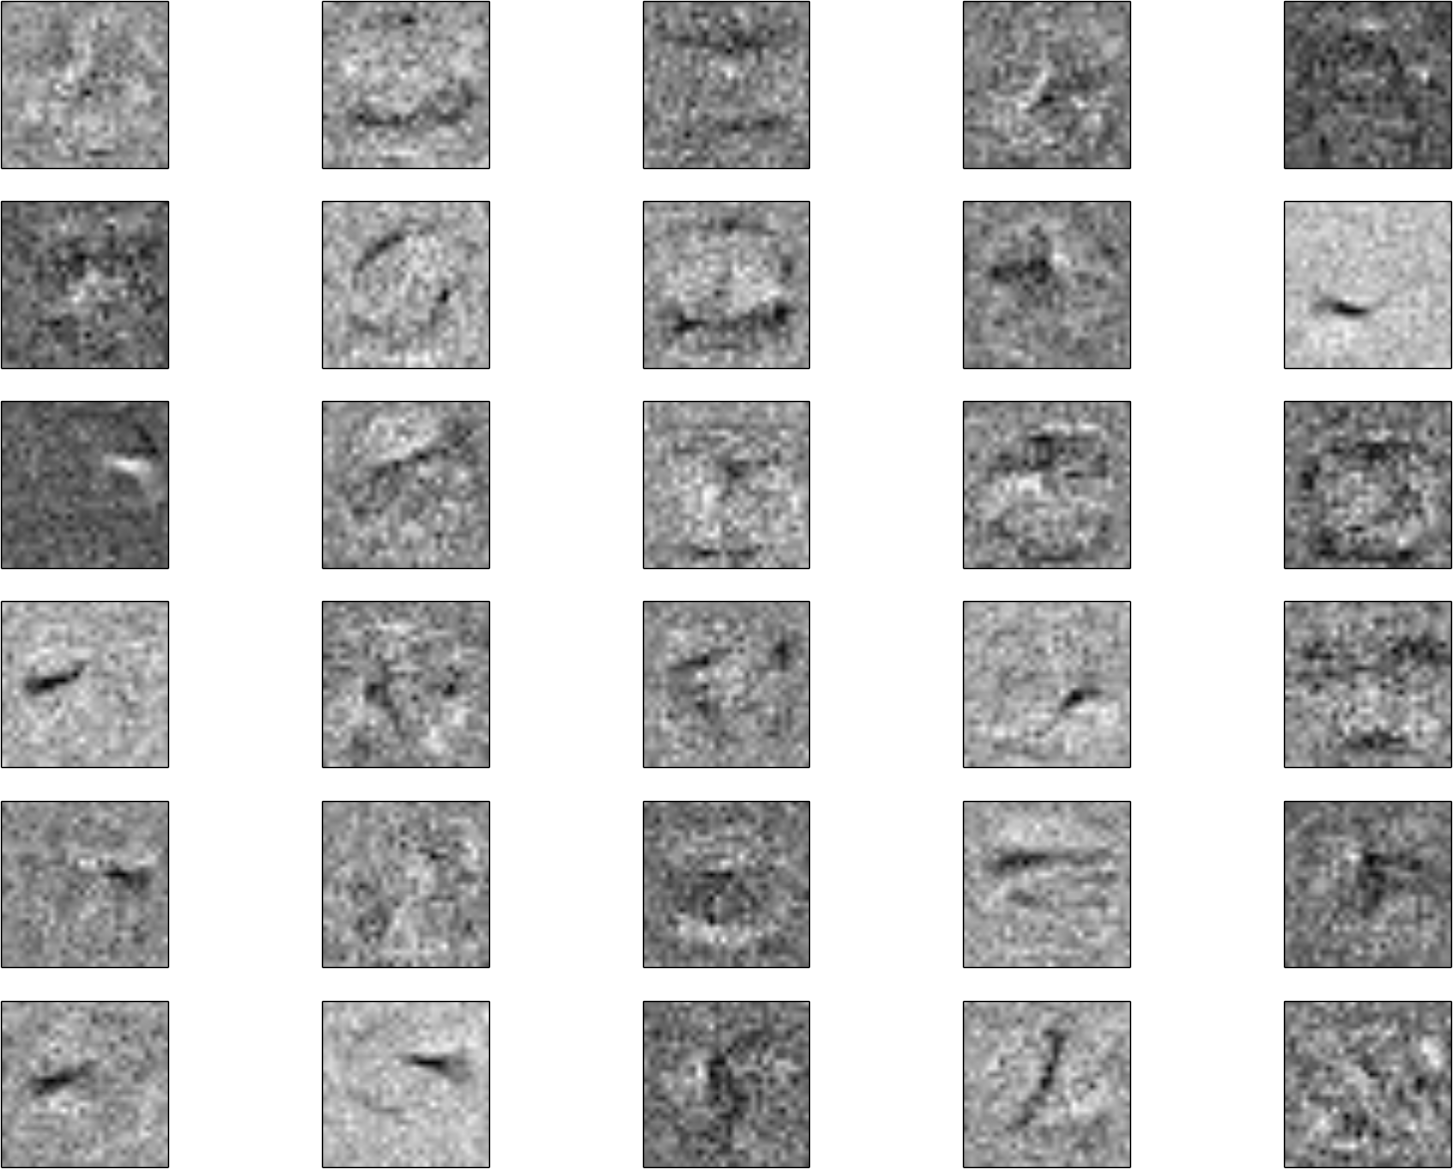
\includegraphics[width=0.8\textwidth]{blick-in-die-zwischenschicht}
  \par
\end{frame}

\note{\justifying
  Hier wurde ein einfaches Netz zur Ziffernerkennung bestehend aus nur einer
  einzigen verborgenen Schicht mit~30 Neuronen trainiert. Die Grafik zeigt die
  Gewichte der Synapsen zwischen den $28 \times 28$ Eingabeneuronen und diesen
  30~Neuronen. Das Netz hat eine Erkennungsrate von~95\,\%.
  \bigskip

  Verwendet man~100 Neuronen, so erreicht man~97\,\%; das ist fast eine
  Halbierung der Fehlerrate.
  \bigskip

  Demo zum Selbstprobieren:
  \begin{itemize}
    \item
    \href{https://github.com/iblech/mathematik-der-vorhersagen/blob/master/neuronale-netze/ziffern/demo.py}{Python-Code
    zur Erkennung}
    \item
    \href{https://github.com/iblech/mathematik-der-vorhersagen/blob/master/neuronale-netze/ziffern/ziffernerkennung-basic.py}{Python-Code
    zum Training}
  \end{itemize}
}


\section[Wieso nicht früher?]{Wieso nicht schon früher?}

{\usebackgroundtemplate{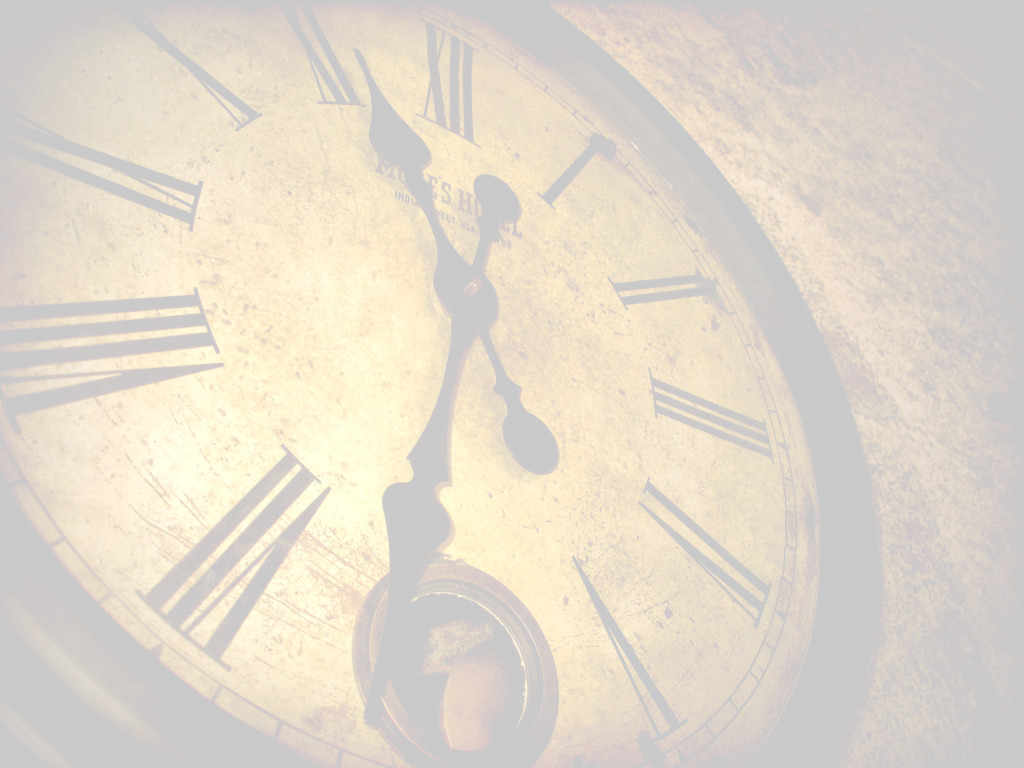
\includegraphics[height=\paperheight]{zeit}}
\begin{frame}
  \centering
  \bigskip\bigskip

  \Huge \hil{Teil III}

  \bigskip
  \Large\textbf{Wieso nicht schon früher?}
  \par

  \vfill\small
  \begin{enumerate}
    \item Größere Rechenleistung
    \pause
    \item Verfügbarkeit großer Datensätze zum Training
    \pause
    \item Mathematischer Durchbruch: Convolutional Neural Networks
  \end{enumerate}
\end{frame}}

% XXX: Bild von CNN einfügen


\section[Weiter?]{Herausforderungen für die Zukunft}

% http://www.bundesheer.at/archiv/a2005/edelweiss_raid/galerie/vollbild/weitergehts2.jpg
{\usebackgroundtemplate{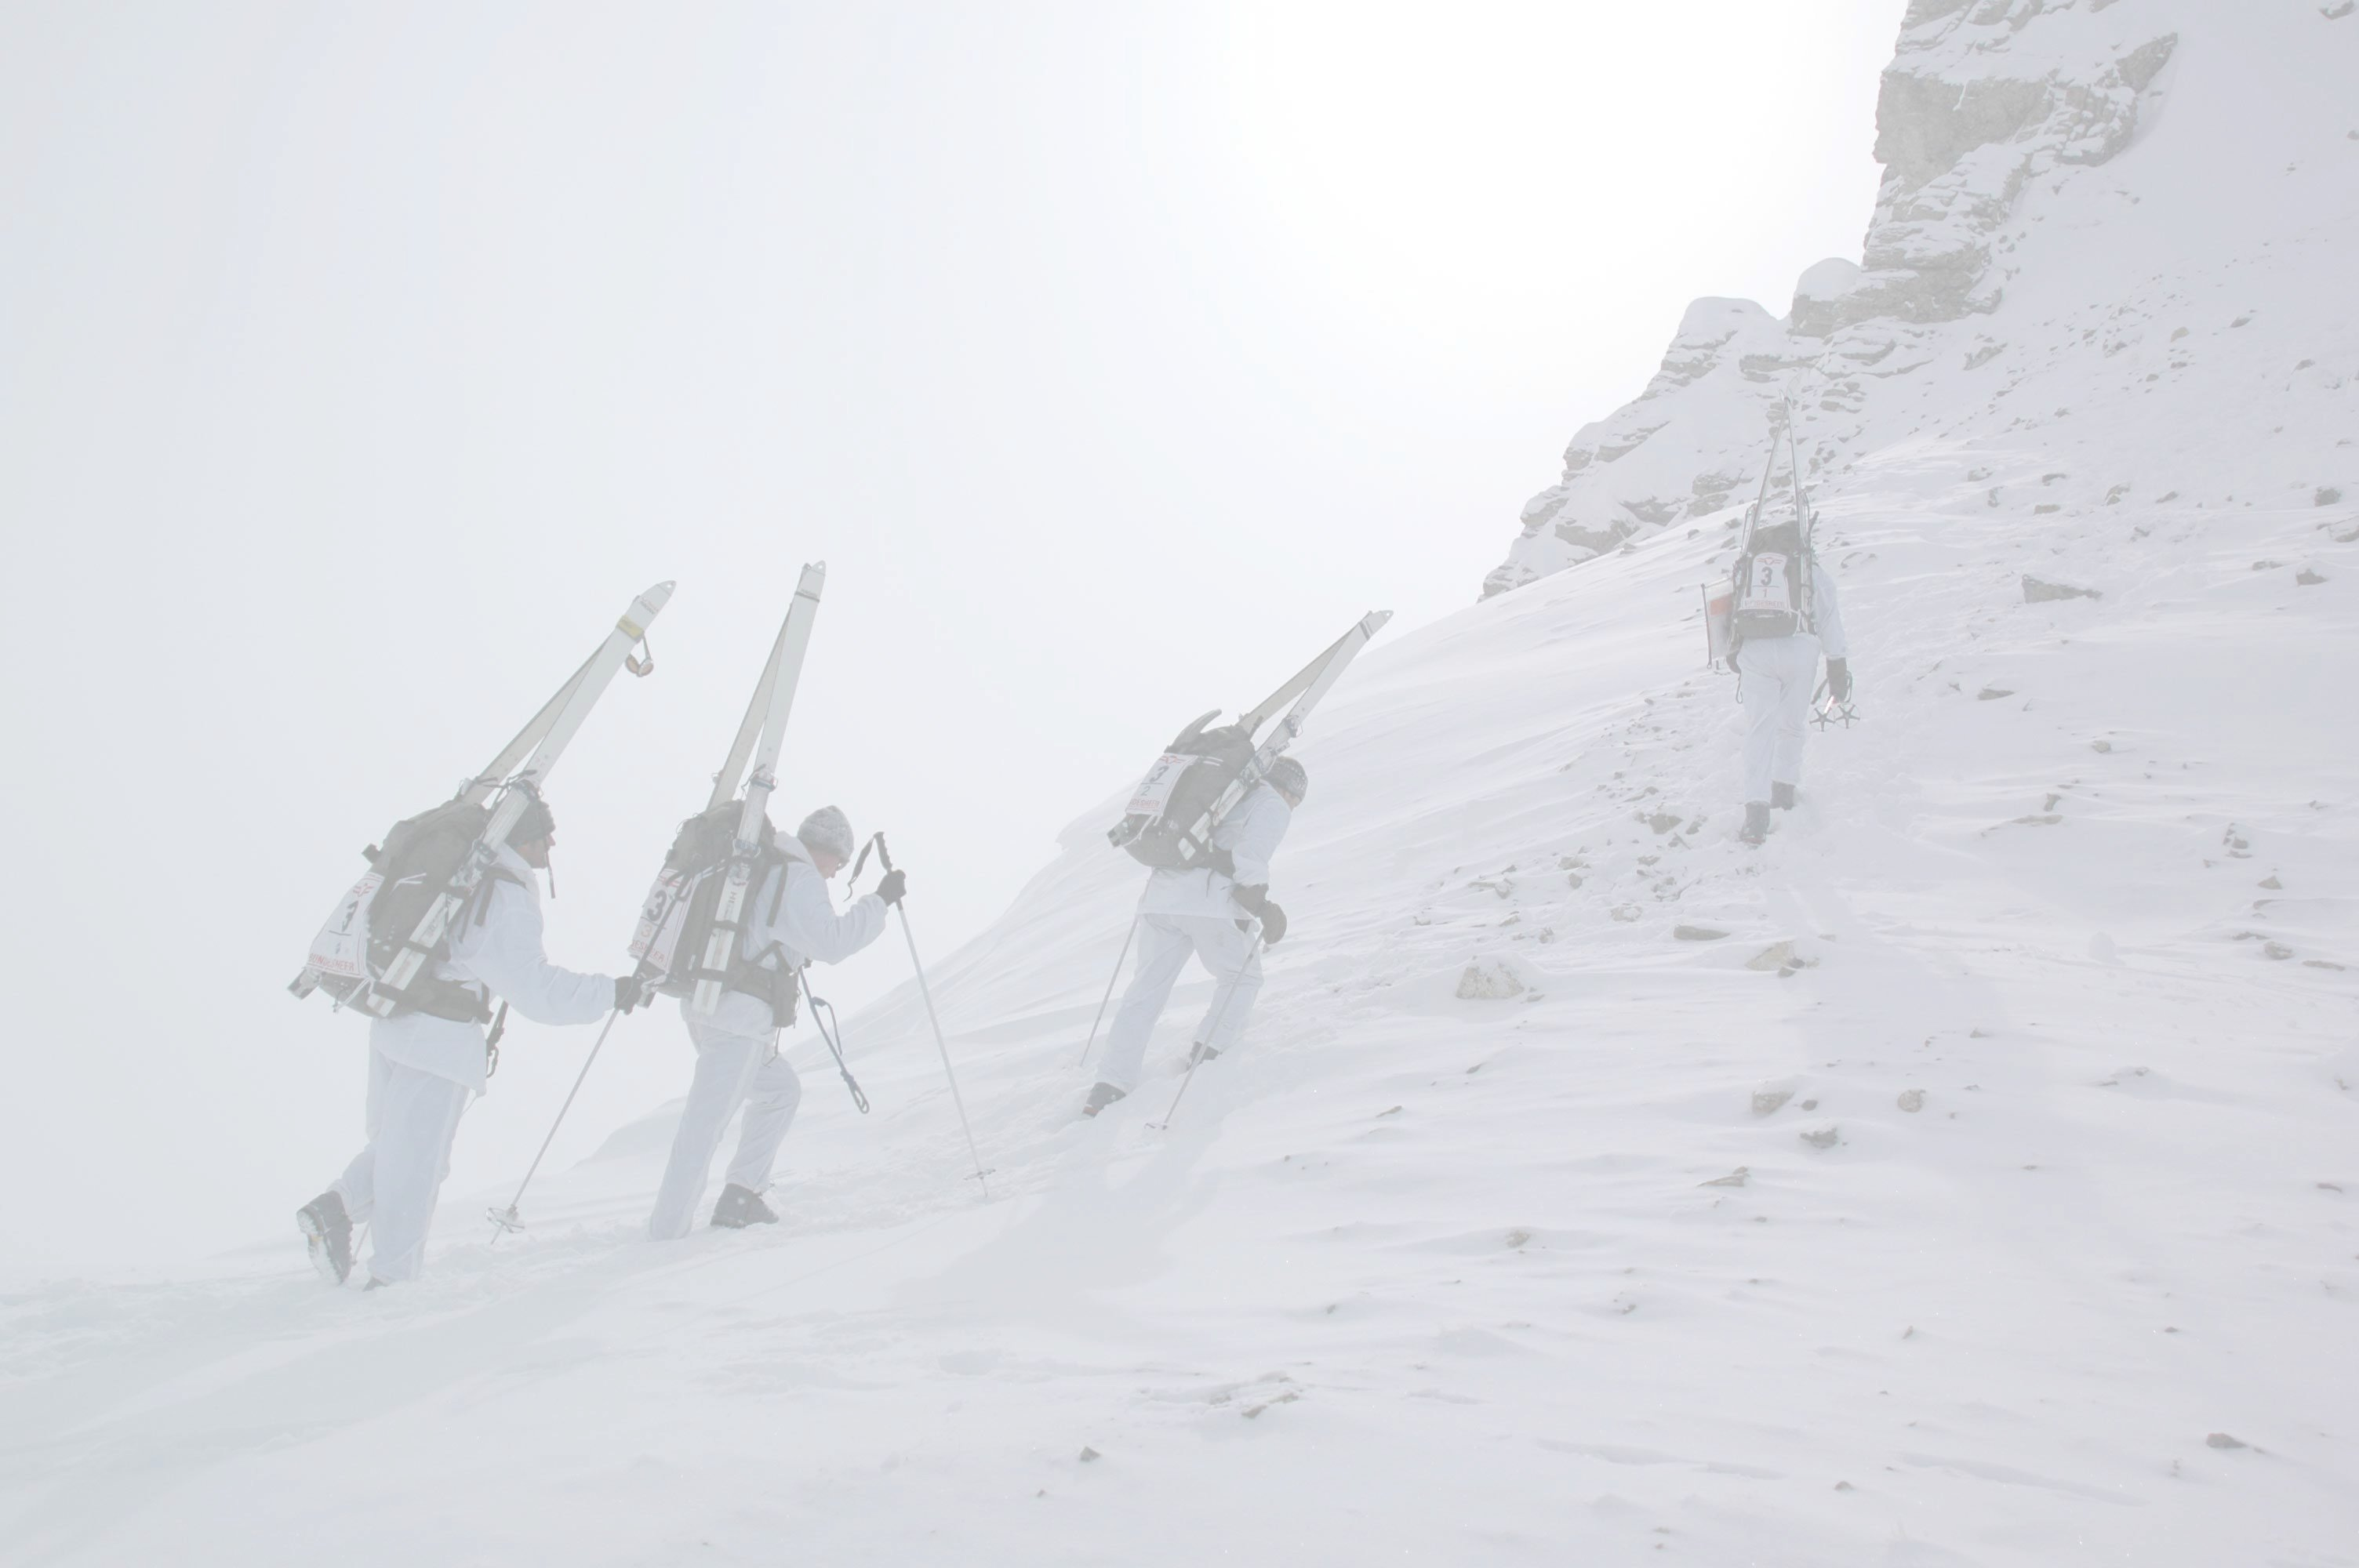
\includegraphics[height=\paperheight]{herausforderung}}
\begin{frame}
  \centering
  \bigskip\bigskip

  \Huge \hil{Teil IV}

  \bigskip
  \Large\textbf{Herausforderungen für die Zukunft}
  \par

  \vfill\small
  \begin{itemize}
    \item Neuronale Netze auf weitere Problemklassen ausdehnen
    \item Innere Funktionsweise von Netzen verstehen
    \item Resistenz gegen \href{https://blog.openai.com/adversarial-example-research/}{Adversarial Examples} entwickeln
    \item Ethische Fragen bei selbstfahrenden Autos diskutieren
    \item Existenzielle Fragen bei starker KI untersuchen
  \end{itemize}
\end{frame}}

\note{\justifying
  \emph{Wie} ein künstliches neuronales Netzwerk funktioniert, ist -- anders
  als bei herkömmlichem Programmcode -- nicht klar.
  (Wie beim Menschen auch.) Dazu wird momentan aktiv geforscht. Zwei
  Einstiegspunkte zu solchen Untersuchungen sind:

  \begin{itemize}
    \item \href{https://research.googleblog.com/2015/06/inceptionism-going-deeper-into-neural.html}{Inceptionism:
    Going Deeper into Neural Networks} von Alexander Mordvintsev, Christopher
    Olah und Mike Tyka
    \item \href{http://www.matthewzeiler.com/pubs/arxive2013/eccv2014.pdf}{Visualizing
    and Understanding Convolutional Networks} von Matthew Zeiler und Rob Fergus
  \end{itemize}
}


\section{Empfehlungen}

{\usebackgroundtemplate{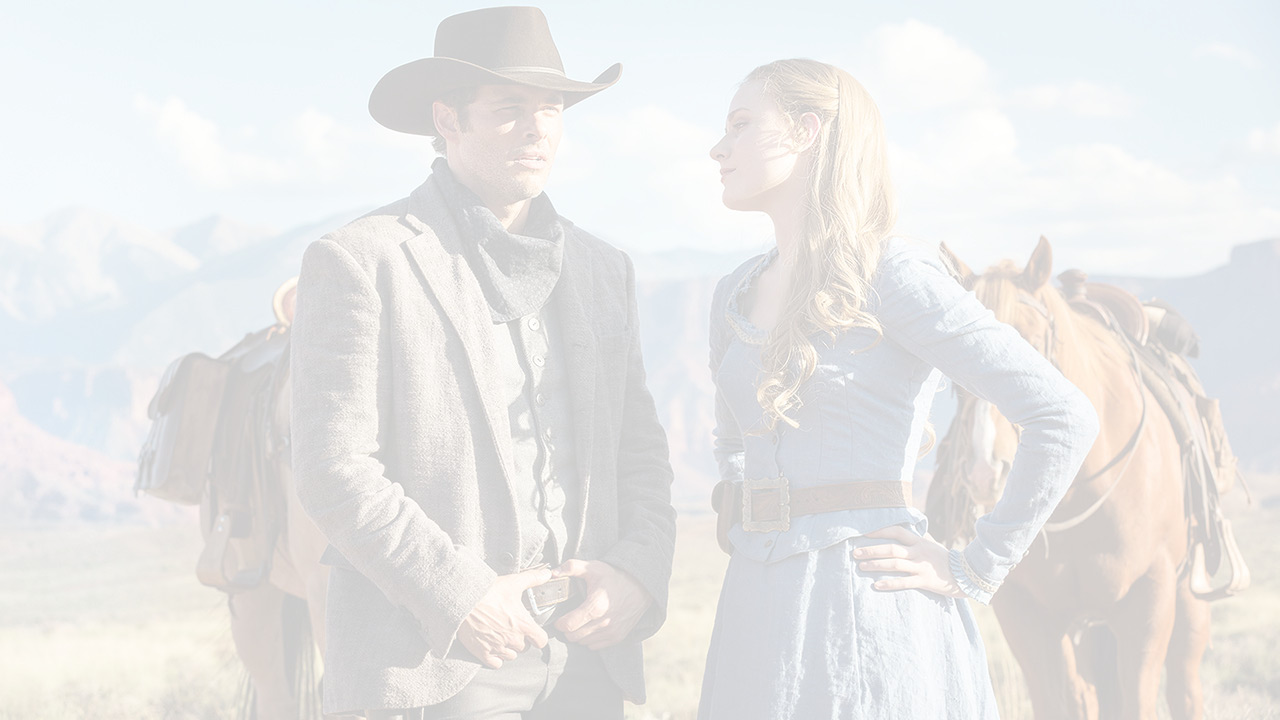
\includegraphics[height=\paperheight]{westworld}}
\begin{frame}
  \centering
  \bigskip\bigskip

  \Huge \hil{Teil V}

  \bigskip
  \Large\textbf{Empfehlungen}
  \par

  \vfill\small
  \begin{itemize}
    \item HBO-Serie Westworld über Androiden, die schon lange den Turingtest
    bestehen und nun ein Bewusstsein entwickeln
    \item \href{https://www.youtube.com/watch?v=lKQ0yaEJjok}{Vorträge von
    Joscha Bach auf dem Kongress}
    \item \href{https://karpathy.github.io/2015/05/21/rnn-effectiveness/}{The
    Unreasonable Effectiveness of Recurrent Neural Networks} von Andrej
    Karpathy
    \item TensorFlow -- mische auch ohne viel Programmiererfahrung bei der
    KI-Entwicklung mit!
    \item \href{http://neuralnetworksanddeeplearning.com/}{Neural Networks and Deep Learning} von Michael Nielsen
  \end{itemize}
\end{frame}}
\end{document}
